\documentclass[11pt,dvipsnames,enabledeprecatedfontcommands]{scrartcl}
\usepackage{lmodern}
\usepackage{amssymb,amsmath}
\usepackage{ifxetex,ifluatex}
\usepackage{fixltx2e} % provides \textsubscript
\ifnum 0\ifxetex 1\fi\ifluatex 1\fi=0 % if pdftex
  \usepackage[T1]{fontenc}
  \usepackage[utf8]{inputenc}
\else % if luatex or xelatex
  \ifxetex
    \usepackage{mathspec}
  \else
    \usepackage{fontspec}
  \fi
  \defaultfontfeatures{Ligatures=TeX,Scale=MatchLowercase}
\fi
% use upquote if available, for straight quotes in verbatim environments
\IfFileExists{upquote.sty}{\usepackage{upquote}}{}
% use microtype if available
\IfFileExists{microtype.sty}{%
\usepackage[]{microtype}
\UseMicrotypeSet[protrusion]{basicmath} % disable protrusion for tt fonts
}{}
\PassOptionsToPackage{hyphens}{url} % url is loaded by hyperref
\usepackage[unicode=true]{hyperref}
\PassOptionsToPackage{usenames,dvipsnames}{color} % color is loaded by hyperref
\hypersetup{
            pdftitle={Rethinking legal probabilism},
            pdfauthor={Rafał Urbaniak},
            colorlinks=true,
            linkcolor=Maroon,
            citecolor=Blue,
            urlcolor=blue,
            breaklinks=true}
\urlstyle{same}  % don't use monospace font for urls
\usepackage{graphicx,grffile}
\makeatletter
\def\maxwidth{\ifdim\Gin@nat@width>\linewidth\linewidth\else\Gin@nat@width\fi}
\def\maxheight{\ifdim\Gin@nat@height>\textheight\textheight\else\Gin@nat@height\fi}
\makeatother
% Scale images if necessary, so that they will not overflow the page
% margins by default, and it is still possible to overwrite the defaults
% using explicit options in \includegraphics[width, height, ...]{}
\setkeys{Gin}{width=\maxwidth,height=\maxheight,keepaspectratio}
\IfFileExists{parskip.sty}{%
\usepackage{parskip}
}{% else
\setlength{\parindent}{0pt}
\setlength{\parskip}{6pt plus 2pt minus 1pt}
}
\setlength{\emergencystretch}{3em}  % prevent overfull lines
\providecommand{\tightlist}{%
  \setlength{\itemsep}{0pt}\setlength{\parskip}{0pt}}
\setcounter{secnumdepth}{5}
% Redefines (sub)paragraphs to behave more like sections
\ifx\paragraph\undefined\else
\let\oldparagraph\paragraph
\renewcommand{\paragraph}[1]{\oldparagraph{#1}\mbox{}}
\fi
\ifx\subparagraph\undefined\else
\let\oldsubparagraph\subparagraph
\renewcommand{\subparagraph}[1]{\oldsubparagraph{#1}\mbox{}}
\fi

% set default figure placement to htbp
\makeatletter
\def\fps@figure{htbp}
\makeatother

%\documentclass{article}

% %packages
 \usepackage{booktabs}

\usepackage{multirow}

\usepackage{graphicx}
\usepackage{longtable}
\usepackage{ragged2e}
\usepackage{etex}
%\usepackage{yfonts}
\usepackage{marvosym}
\usepackage[notextcomp]{kpfonts}
\usepackage{nicefrac}
\newcommand*{\QED}{\hfill \footnotesize {\sc Q.e.d.}}
\usepackage{floatrow}

\usepackage[textsize=scriptsize, textwidth = 1.5cm]{todonotes}
%\linespread{1.5}


\setlength{\parindent}{10pt}
\setlength{\parskip}{1pt}


%language
\usepackage{times}
\usepackage{t1enc}
%\usepackage[utf8x]{inputenc}
%\usepackage[polish]{babel}
%\usepackage{polski}

\usepackage{mathptmx}
\usepackage[scaled=0.88]{helvet}


%AMS
\usepackage{amsfonts}
\usepackage{amssymb}
\usepackage{amsthm}
\usepackage{amsmath}
\usepackage{mathtools}

\usepackage{geometry}
 \geometry{a4paper,left=20mm,top=15mm,bottom = 15mm, right = 20mm}


%environments
\newtheorem{fact}{Fact}



%abbreviations
\newcommand{\ra}{\rangle}
\newcommand{\la}{\langle}
\newcommand{\n}{\neg}
\newcommand{\et}{\wedge}
\newcommand{\jt}{\rightarrow}
\newcommand{\ko}[1]{\forall  #1\,}
\newcommand{\ro}{\leftrightarrow}
\newcommand{\exi}[1]{\exists\, {_{#1}}}
\newcommand{\pr}[1]{\mathsf{P}(#1)}
\newcommand{\cost}{\mathsf{cost}}


\newcommand{\odds}{\mathsf{Odds}}
\newcommand{\ind}{\mathsf{Ind}}
\newcommand{\nf}[2]{\nicefrac{#1\,}{#2}}
\newcommand{\R}[1]{\texttt{#1}}
\newcommand{\prr}[1]{\mbox{$\mathtt{P}_{prior}(#1)$}}
\newcommand{\prp}[1]{\mbox{$\mathtt{P}_{posterior}(#1)$}}



\newtheorem{q}{\color{blue}Question}
\newtheorem{lemma}{Lemma}
\newtheorem{theorem}{Theorem}



%technical intermezzo
%---------------------

\newcommand{\intermezzoa}{
	\begin{minipage}[c]{13cm}
	\begin{center}\rule{10cm}{0.4pt}



	\tiny{\sc Optional Content Starts}
	
	\vspace{-1mm}
	
	\rule{10cm}{0.4pt}\end{center}
	\end{minipage}\nopagebreak 
	}


\newcommand{\intermezzob}{\nopagebreak 
	\begin{minipage}[c]{13cm}
	\begin{center}\rule{10cm}{0.4pt}

	\tiny{\sc Optional Content Ends}
	
	\vspace{-1mm}
	
	\rule{10cm}{0.4pt}\end{center}
	\end{minipage}
	}
%--------------------

\DeclareUnicodeCharacter{0301}{*************************************}




















\newtheorem*{reply*}{Reply}
\usepackage{enumitem}
\newcommand{\question}[1]{\begin{enumerate}[resume,leftmargin=0cm,labelsep=0cm,align=left]
\item #1
\end{enumerate}}

\usepackage{float}

% \setbeamertemplate{blocks}[rounded][shadow=true]
% \setbeamertemplate{itemize items}[ball]
% \AtBeginPart{}
% \AtBeginSection{}
% \AtBeginSubsection{}
% \AtBeginSubsubsection{}
% \setlength{\emergencystretch}{0em}
% \setlength{\parskip}{0pt}






\usepackage[authoryear]{natbib}

%\bibliographystyle{apalike}

\title{Rethinking legal probabilism}
\author{Rafał Urbaniak}
\date{}

\begin{document}
\maketitle

\thispagestyle{empty}

\section{Scientific goal}\label{scientific-goal}

As many miscarriages of justice indicate, scientific evidence is easily
misinterpreted in court. This happens partially due to miscommunication
between the parties involved, partially due to the usual probabilistic
fallacies, but also because incorporating scientific evidence in the
context of a whole case can be really hard. While probabilistic tools
for piecemeal evaluation of scientific evidence and spotting
probabilistic fallacies in legal contexts are quite well
developed,\todo{say sth about replicability crisis in forensic sciences at some point?}
the construction of a more general probabilistic model of incorporating
such evidence in a wider context of a whole case, probabilistic
explication of and theorizing about evidence evaluation and legal
decision standards, remain a challenge. Legal probabilism (LP), for our
purpose, is the view that this challenge can and should be met. This
project intends to contribute to further development of this enterprise
in a philosophically motivated manner.

The assessment of evidence in the court of law can be viewed from at
least three perspectives: as an interplay of arguments, as an assessment
of probabilities involved, or as an interaction of competing narrations.
Each perspective presents an account of legal reasoning (Di Bello \&
Verheij, 2018; van Eemeren \& Verheij, 2017). Individually, each of
these strains has been investigated. The probabilistic approach is the
most developed one but LP is still underdeveloped ---to a large extent
this is so in light of various lines of criticism developed by the
representatives of the other strains.

The \textbf{goal of this project} is to contribute to the
\textbf{development of legal probabilism} by formulating its variant
that accomodates important \textbf{insights provided by its critics}. A
crucial point of criticism is that the fact-finding process should be
conceptualized as \textbf{a competition of narrations}. I plan to
develop methods that allow the probabilist to take this perspective, and
explain how such methods allow the legal probabilist to address various
objections present in the literature. The key idea is that once
\textbf{narrations are represented as bayesian networks, various criteria on,  features of  and operations on narrations can be explicated in terms of corresponding properties of and operations on bayesian networks}.
Further, the hypothesis is that such an improved framework will
facilitate addressing key objections raised against LP.

The conceptual developments will be accompanied by technical accounts.
\textbf{\textsf{R}} code capturing the technical features developed will
be made available to the reader. Thus, the output will be a
\textbf{unifying extended probabilistic model embracing key aspects of the narrative and argumentative approaches, susceptible to AI implementation.}
The methods employed include: Bayesian statistical methods (including
Bayesian approach to higher-order probability), imprecise probabilities,
and Bayesian networks.

\newpage 

\tableofcontents

\newpage

\section{Significance}\label{significance}

\footnotesize \emph{
(state of the art, justification for tackling a specific scientific problem,
justification for the pioneering nature of the project,
the impact of the project results on the development of the research field and scientific discipline);
} \normalsize

\subsection{State of the art}\label{state-of-the-art}

\subsubsection{Legal probabilisim}\label{legal-probabilisim}

One of the functions of the trial is to resolve disputes about questions
of facts. Did the defendant rob the bank? Who is the father of the
child? Did this drug cause birth defects? To answer such questions, the
litigants will present evidence of different kinds: eyewitness
testimonies, DNA matches, epidemiological studies, etc. The evidence
presented will often be in conflict with other evidence. In a bank
robbery case, for example, the prosecution may present eyewitness
testimony that the defendant was seen driving a truck near the bank a
few minutes after the robbery took place. The defense may respond that
no traces were found at the crime scene that would match the defendant.
The fact-finders, judges or lay jurors, should address these conflicts
by assessing and weighing the evidence, and on that basis reach a final
decision. This is a difficult task. The evidence presented at trial can
be complex and open to multiple interpretations, and even when it is
assessed carefully, it may still lead to an incorrect verdict. How
should judges and jurors respond to this uncertainty?

From among the three perspectives mentioned in the beginning, the
probablistic approach will be my point of departure, for the following
key reasons:

\begin{itemize}
\item
  The project is to be informed by and reflect on the actual practice of
  legal evidence evaluation, and much of scientific evidence in such
  contexts has probabilistic form.
\item
  Probabilistic tools are fairly well-developed both for applications
  and within formal epistemology, reaching a state of fruition which
  should inspire deeper reflection.
\item
  Statistical computing tools for such methods are available, which
  makes programming development and preliminary computational and
  data-driven evaluation of the ideas to be defended a viable
  enterprise.
\end{itemize}

Accoringly, the view in focus of this research is legal probabilism
(LP)---an ongoing research program that comprises a variety of claims
about evidence assessment and decision-making at trial. At its simplest,
it comprises two core tenets: first, that the evidence presented at
trial can be assessed, weighed and combined by means of probability
theory; and second, that legal decision rules, such as proof beyond a
reasonable doubt in criminal cases, can be explicated in probabilistic
terms.

In the Middle Ages, before the advent of probability theory, there
existed an informal mathematics of legal evidence (Wigmore, 1901).
Formalistic procedures fixed the number of witnesses required to
establish a claim. Lawyers would list ways in which items of evidence
could be added or subtracted to weaken or strengthen one's case. This
formalistic system fell into disrepute as the Enlightenment principle of
`free proof' gained wide acceptance (Damaška, 1995). Concurrently, the
development of probability theory brought forth a new approach to
weighing evidence and making decisions under uncertainty. The early
theorists of probability in the 17th and 18th century were as much
interested in games of chance as they were interested in the uncertainty
of trial decisions (Daston, 1988; Franklin, 2001; Hacking, 1975).
Bernoulli (1713) was one of the first to formulate probabilistic rules
for combining different pieces of evidence in legal cases and assessing
to what extent they supported a claim of interest. He was also one of
the first to suggest that decision rules at trial could be understood as
probability thresholds.

Bernoulli's prescient insights attained greater popularity in the 20th
century amidst the law and economics movement (Becker, 1968; Calabresi,
1961; Posner, 1973). In a seminal article, Finkelstein \& Fairley (1970)
gave one of the first systematic analyses of how probability theory, and
Bayes' theorem in particular, can help to weigh evidence at trial.
Lempert (1977) was one of the first to rely on probability theory,
specifically likelihood ratios, for assessing the relevance of evidence.
Such contributions fueled what has been called the New Evidence
Scholarship, a rigorous way of studying the process of legal proof at
trial (Lempert, 1986).

\subsubsection{Skeptical voices and
challenges}\label{skeptical-voices-and-challenges}

In response to such developments, Tribe (1971) attacked what he called
`trial by mathematics'. His critique ranged from listing well-known
cases of misuse or probabilities in legal contexts and practical
difficulties in assessing the probability of someone's criminal or civil
liability to the dehumanization of trial decisions. After Tribe, many
have criticized legal probabilism on a variety of grounds, both
theoretical and practical, arguing that probabilistic models are either
inadequate or unhelpful (Brilmayer, 1986; Cohen, 1986; Dant, 1988, Allen
(1986); Underwood, 1977).

After the discovery of DNA fingerprinting in the eighties, many legal
probabilists focused on how probability theory could be used to quantify
the strength of a DNA match under various circumstances (Kaye, 1986,
2010; Koehler, 1996; National Research Council, 1992; Robertson \&
Vignaux, 1995).

Some legal scholars and practitioners have voiced their support for
legal probabilism explicitly (Tillers \& Gottfried, 2007). Yet
skepticism about mathematical and quantitative models of legal evidence
is still widespread among prominent legal scholars and practitioners
(see, for example, Allen \& Pardo, 2007). Even among legal probabilists,
few would think it possible to quantify precisely the probability of
someone's guilt or civil liability. In response, probabilistists such as
Taroni, Biedermann, Bozza, Garbolino, \& Aitken (2014) suggest that the
probabilistic formalism is still useful as an aid to structure and guide
one's inferences under uncertainty, rather than a way to reach precise
numerical assessments.

Conceptually, the probabilistic approach togehter with
decision-theoretic considerations, can be used to theorize about the
standard of proof and its properties. But for this project to be
successfull, a proper probabilist explication of such a standard needs
to be agreed upon. Imagine you are a trier of fact in a legal proceeding
in which the defendant's guilt is identified as equivalent to a certain
factual statement \(G\) and that somehow you succeeded in properly
evaluating \(\pr{G\vert E}\)----the probability of \(G\) given the total
evidence presented to you, \(E\) One question that arises in such a
situation is: when should you decide against the defendant? when is the
evidence good enough? What we are after here is a condition \(\Psi\),
formulated in (primarily) probabilistic (and perhaps decision-theoretic)
terms, such that the trier of fact, at least ideally, should accept any
relevant claim \(A\) (including \(G\)) just in case \(\Psi(A, E)\). One
straightforward attempt might be to say: convict if \(\pr{G\vert E}\) is
above a certain threshold, otherwise acquit.

Perhaps the most difficult conceptual challenge to such probabilistic
explications---at least, one that has galvanized philosophical attention
in recent years---comes from the paradoxes of legal proof or puzzles of
naked statistical evidence. In a number of seminal papers, Nesson
(1979), Cohen (1981), and Thomson (1986) formulated scenarios in which,
even if the probability of guilt or civil liability, based on the
available evidence, is particularly high, a verdict against the
defendant seems unwarranted.

A variant of such a scenario---the gatecrasher paradox---goes as
follows. Suppose our guilt threshold is high, say at 0.99. Consider the
situation in which 1000 fans enter a football stadium, and 991 of them
avoid paying for their tickets. A random spectator is tried for not
paying. The probability that the spectator under trial did not pay
exceeds 0.99. Yet,intuitively, a spectator cannot be considered liable
on the sole basis of the number of people who did and did not pay.

Another problem with the proposal is the so-called difficulty about
conjunction. It arises, because intuitively there should be no
difference between the trier's acceptance of \(A\) and \(B\) separately,
and her acceptance of their conjunction, \(A\wedge B\) , that is, that
\(\Psi(A,E)\) and \(\Psi(B,E)\) just in case \(\Psi(A\wedge B, E)\). If
\(\Psi(H,E)\) just the threshold criterion, requiring that
\(\pr{H\vert E}\) be sufficiently high, \(\Psi\) in general fails to
satisfy this equivalence.

Arguably, these scenarios underscore a theoretical difficulty with
probabilistic accounts of legal standards of proof. Many articles have
been written on the topic, initially by legal scholars. In the last
decade, philosophers have also joined the debate---for critical surveys
see Redmayne (2008), Gardiner (2018) and Pardo (2019). Crucially, even
fairly recent proposals to mend the situation (Dawid, 1987, Cheng
(2012), Kaplow (2014)) on the part of the legal probabilist have failed
(Urbaniak, 2019 contains a detailed analysis).

At least \emph{prima facie}, then, it seems that some conditions other
than high posterior probability of liability have to be satisfied for
the decision to penalize (or find liable) to be justified. Accordingly,
various informal notions have been claimed to be essential for a proper
explication of judiciary decision standards (Haack, 2014; Wells, 1992).
For instance, evidence is claimed to be insufficient for conviction if
it is not \emph{sensitive} to the issue at hand: if it remained the same
even if the accused was innocent (Enoch \& Fisher, 2015). Or, to look at
another approach, evidence is claimed to be insufficient for conviction
if it doesn't \emph{normically support} it: if---given the same
evidence---no explanation would be needed even if the accused was
innocent (Smith, 2017). A legal probabilist needs either to show that
these notions are unnecessary or inadequate for the purpose at hand, or
to indicate how they can be explicated in probabilistic terms.

\subsubsection{The narrative approach}\label{the-narrative-approach}

More recently, alternative frameworks for modeling evidential reasoning
and decision-making at trial have been proposed. They are based on
inference to the best explanation (Allen, 2010; Pardo \& Allen, 2008),
narratives and stories (Allen, 1986, 2010; Allen \& Leiter, 2001;
Clermont, 2015; Pardo, 2018; Pennington \& Hastie, 1991a), and
argumentation theory (Bex, 2011; Gordon, Prakken, \& Walton, 2007;
Walton, 2002). Those who favor a conciliatory stance have combined legal
probabilism with other frameworks, offering preliminary sketches of
hybrid theories (Urbaniak, 2018; Verheij, 2014).

Another important point of criticism of LP is that legal proceedings are
back-and-forth between opposing parties in which cross-examination is of
crucial importance, reasoning goes not only evidence-to-hypothesis, but
also hypotheses-to-evidence (Allen \& Pardo, 2007; Wells, 1992) in a way
that seems analogous to inference to the best explanation (Dant, 1988),
which notoriously is claimed to not be susceptible to probabilistic
analysis (Lipton, 2004). An informal philosophical account inspired by
such considerations---The \textbf{No Plausible Alternative Story (NPAS)}
theory (Allen, 2010)---is that the courtroom is a confrontation of
competing narrations (Ho, 2008; Wagenaar, Van Koppen, \& Crombag, 1993)
offered by the sides, and the narrative to be selected should be the
most plausible one. The view is conceptually plausible (Di Bello, 2013),
and finds support in psychological evidence (Pennington \& Hastie,
1991b, 1992).

It would be a great advantage of legal probabilism if it could model
phenomena captured by the narrative approach. But how is the legal
probabilist to make sense of them? From her perspective, the key
disadvantage of NPAS is that it abandons the rich toolbox of
probabilistic methods and takes the key notion of plausibility to be a
primitive notion which should be understood only intuitively.

\subsubsection{Bayesian networks as a tool for legal
probabilism}\label{bayesian-networks-as-a-tool-for-legal-probabilism}

The idea that Bayesian networks can be used for probabilistic reasoning
in legal fact-finding started gaining traction in late eighties and
early nineties (Edwards, 1991), and it found its way to nowadays
standard textbooks on the topic (Fenton \& Neil, 2018; Taroni et al.,
2014).\\
A Bayesian network comprises two components: first, a directed acyclic
graph of relations of dependence (represented by arrows) between
variables (represented by nodes); second, conditional probability
tables. Consider the graphical component first. The graph is acyclic
because the arrows connecting the nodes do not form loops. As an
illustration, let \(H\) be the claim that the suspect committed the
murder, \(BT\) the presence of a blood type B match with a crime scene
stain, and \(W\) the fact that an eyewitness observed the suspect near
the scene around the time of the crime. The graphical component of the
Bayesian network would look like this:

\begin{center}\includegraphics{BNfiles/unnamed-chunk-2-1} \end{center}

The \emph{ancestors} of a node \(X\) are all those nodes from which we
can reach \(X\) by following the arrows going forwards. The
\textit{parents} of a node \(X\) are those for which we can do this in
one step. The \textit{descendants} of \(X\) are all which can be reached
from \(X\) by following the arrows going forward. The \textit{children}
are those for which we can do this in one step. In the example, \(H\) is
the parent (and ancestor) of both \$ W\$ and \(BT\), which are its
children (and descendants). There are no non-parent ancestors or
non-children descendants.

The variables, which are represented by nodes and are connected by
arrows, stand in relation of probabilistic dependence. To describe these
relations, the graphical model is accompanied by conditional probability
tables. For parentless nodes such as \(H\), the tables specify the prior
probabilities of all their possible states. Assuming \(H\) stands for a
binary random variable, with two possible states, the prior
probabilities could be:

\begin{table}[H]
\centering
\begin{tabular}{lr}
\toprule
  & Prior\\
\midrule
H=murder & .01\\
H=no.murder & .99\\
\bottomrule
\end{tabular}
\end{table}

\noindent
The .01 figure for H=murder rests on the assumption that, absent any
incriminating evidence, the defendant is unlikely to be guilty. For
children nodes, the tables specify their conditional probability given
combinations of their parents' states. If the variables are binary, an
assignment of values for them could be:

\begin{table}[H]
\centering
\begin{tabular}{lrr}
\toprule
  & H=murder & H=no.murder\\
\midrule
W=seen & .7 & .4\\
W=not.seen & .3 & .6\\
\bottomrule
\end{tabular}
\end{table}

\begin{table}[H]
\centering
\begin{tabular}{lrr}
\toprule
  & H=murder & H=no.murder\\
\midrule
BT=match & 1 & .063\\
BT=no.match & 0 & .937\\
\bottomrule
\end{tabular}
\end{table}

\noindent
According to the tables above, even if the defendant is not the culprit,
the eyewitness testimony would still incriminate him with probability of
.4, while the blood evidence with probability equal to only .063. The
blood type frequency estimate is realistic (Lucy, 2013), and so are the
conditional probabilities for the eyewitness identification. As
expected, eyewitness testimony is assumed to be less trustworthy than
blood match evidence (Urbaniak, Kowalewska, Janda, \&
Dziurosz-Serafinowicz, 2020; but for complications about assessing
eyewitness testimony, see Wixted \& Wells, 2017).

The three probability tables above are all that is needed to define the
probability distribution. The tables do not specify probabilistic
dependencies between nodes that are not in a relation of child/parent,
such as \(BT\) and \(W\). Since there is no arrow between them, nodes
\(BT\) and \(W\) are assumed to be independent conditional on \(H\),
that is, \(\pr(W \vert H)=\pr(W \vert H \wedge BT)\). This fact
represents, as part of the structure of the network, the independence
between eyewitness testimony and blood evidence. A generalization of
this fact is the so-called Markov condition. While the Bayesian network
above---comprising a directed acyclic graph along with probability
tables---is simple, a correct intuitive assessment of the probability of
the hypothesis given the evidence is already challenging. The reader is
invited to try to estimate intuitively the probability that the
defendant committed the murder (H=murder) given the following states of
the evidence:

\begin{itemize} 
\item The suspect's blood type matches the crime stain but  information about the witness is unavailable.
\item The suspect's blood type matches the crime stain but the witness says they did not see the suspect near the crime scene.
\item The suspect's blood type matches the crime stain and the witness says they saw the suspect near the crime scene.
\end{itemize}

\noindent Already at this level of complexity, calculations by hand
become cumbersome. In contrast, software for Bayesian networks (see, for
example, the \(\textbf{\textsf{R}}\) package
\(\textbf{\textsf{bnlearn}}\) developed by Marco Scutari and described
in Scutari \& Denis, 2015) will easily give the following results:

\begin{table}[H]
\centering
\begin{tabular}{lr}
\toprule
  & H=murder\\
\midrule
BT=match,W=? & .138\\
BT=match,W=not.seen & .074\\
BT=match, W=seen & .219\\
\bottomrule
\end{tabular}
\end{table}

\noindent
Perhaps surprisingly the posterior probability of \(H\) is about .22
even when both pieces of evidence are incriminating (BT=match, W=seen).

Simple graphical patterns (called \emph{idioms}) often recur while
modeling the relationships between evidence and hypotheses. Complex
graphical models can be created by combining these basic patters in a
modular way. Discussion of general methods for Bayesian network
constructions can be found in (Neil, Fenton, \& Nielson, 2000), (Hepler,
Dawid, \& Leucari, 2007) and general idioms are discussed in (Fenton,
Neil, \& Lagnado, 2013). As an example, consider the
\emph{evidence idiom} is the most basic graphical representation of the
relation between a hypothesis and a piece of evidence:

\begin{center}\includegraphics{BNfiles/unnamed-chunk-6-1} \end{center}

\noindent  This directed graph suggests that the direction of
influence---which could, but need not, be interpreted as causal
influence---goes from hypothesis to evidence (though the probabilistic
dependence goes both ways). The hypothesis node and the evidence node
can be binary variables, such as ``The defendant was the source of the
crime scene traces'' (hypothesis) and ``The defendant genetically
matches the crime traces'' (evidence). But the variables need not be
binary. The hypothesis node might take values from the range of
\(1-40\), say the distance in meters from which the gun was shot, and
the evidence node might be a continuous variable representing the
density of gun shot residues (Taroni et al., 2014).

As an example of a more complex idiom, called the
\emph{evidence accuracy
idiom}, consists of two arrows going into the evidence node {[}Bovens \&
Hartmann (2004); friedman1974{]}. One incoming arrow comes from the
hypothesis node and the other from the accuracy node. This idiom can be
used to model, say, an alcohol test:

\begin{center}\includegraphics{BNfiles/unnamed-chunk-7-1} \end{center}

\noindent The directions of the arrows indicate that the accuracy of the
evidence (accuracy node) and the alcohol level (hypothesis node)
influence the outcome of the test (evidence node). The graphical model
represents different sources of uncertainty. The uncertainty associated
with the sensitivity and specificity of the test---that is, the
probability that the tests reports excessive alcohol level when the
level is excessive (sensitivity) and the probability that the test
reports normal alcohol level when the level is normal (specificity)---is
captured by the arrow going from the hypothesis node
(\textsf{Excess alcohol level}) to the evidence node
(\textsf{Evidence for excess}). Other sources of uncertainty comprise
the possibility that the police officer lied about the test report or
the possibility that the driver took medications which then affected the
alcohol level. These possibilities can be taken into consideration by
adding an accuracy node (or multiple accuracy nodes, if each factor is
kept separate from the other).

The key poin there is that large steps have been made towards the
development of BN-related tools for evidence evaluation. However, so
far, most of them have to do with presentation and evaluation of various
pieces of evidence, not with the development of a more general model to
facilitate more general probabilistic reflection on legal decision
standards.

\subsection{Pioneering nature of the
project}\label{pioneering-nature-of-the-project}

\subsubsection{Key elements of the
approach}\label{key-elements-of-the-approach}

For the reasons already mentioned, Bayesian Networks and probabilistic
methods will be in the focus of this project. It is quite clear that BNs
are useful tool when it comes to piecemeal modeling and evaluation of
scientific evidence in court. The question is, whether they can be
useful for modeling whole cases and casting light on both the conceptual
challenges that we already mention and for incorporating the points made
by the representatives of other strains of research, most crucially, the
NPAS.

Attempts have been made to use Bayesian networks to weigh and assess
complex bodies of evidence consisting of multiple components. On one
hand, we have serious reconstructions of real complex cases. Kadane \&
Schum (2011) made one the first attempts to model an entire criminal
case, Sacco \& Vanzetti from 1920, using probabilistic graphs. More
recently, Fenton \& Neil (2018) constructed a Bayesian network for the
famous Sally Clark case:

\begin{center}\includegraphics{BNfiles/unnamed-chunk-11-1} \end{center}

\noindent
The arrows depict relationships of influence between variables. Whether
Sally Clark's sons, call them \(A\) and \(B\), died by SIDS or murder
(\textsf{A.cause} and \textsf{B.cause}) influences whether signs of
disease (\textsf{A.disease} and \textsf{B.disease}) and bruising
(\textsf{A.bruising} and \textsf{B.bruising}) were present. Since son A
died first, whether A was murdered or died by SIDS (\textsf{A.cause})
influences how son B died (\textsf{B.cause}). How the sons died
determines how many sons were murdered (\textsf{No.murdered}), and how
many sons were murdered decides whether Sally Clark is guilty
(\textsf{guilty}).

According to the calculation by \cite{Fenton2018Risk}, the prior
probability of \textrm{Guilty = Yes} should be .0789. After taking into
account the incriminating evidence presented at trial, such as that
there were signs of bruising but no signs of a preexisting disease
affecting the children, the posterior probabilities are as follows:

\begin{center}
\begin{tabular}{@{}ll@{}}
\toprule
Evidence (cumulative) & $\pr(\textrm{Clark guilty})$ 
\\ \midrule 
A bruising& .2887\\
A no signs of disease & .3093\\
B bruising & .6913\\
B no signs of disease  & .7019\\
 \bottomrule
\end{tabular}
\end{center}

\noindent  The incriminating evidence, combined, brings the probability
of guilt from .0789 to .7019. This is a significant increase, but not
quite enough for a conviction. If one wishes to perform sensitivity
analysis by modifying some of the probabilities, this can be easily
done. During the appeal trial, new evidence was discovered, in
particular, evidence that son A was affected by a disease. Once this
evidence is taken into account, the probability of guilt drops to .00459
(and if signs of disease were also present on B, the guilt probability
would drop even further to .0009). For a general discussion on how to
elicit probabilities, see (Renooij, 2001) and (Gaag, Renooij, Witteman,
Aleman, \& Taal, 2013).

On the other hand, we have more general methodological reflection on the
use of BNs for modeling whole cases. The main idea is that once all the
pieces of evidence and claims are represented as nodes, one should use
the \textit{scenario idiom} to model complex hypotheses, consisting of a
sequence of events organized in space and time: a scenario (Vlek,
Prakken, Renooij, \& Verheij, 2014). A graphical model that uses the
scenario idiom would consist of the following components: first, nodes
for the states and events in the scenario, with each node linked to the
supporting evidence; second, a separate scenario node that has states
and events as its children; finally, a node corresponding to the
ultimate hypothesis as a child of the scenario node. The graphical model
would look like this:

\begin{center}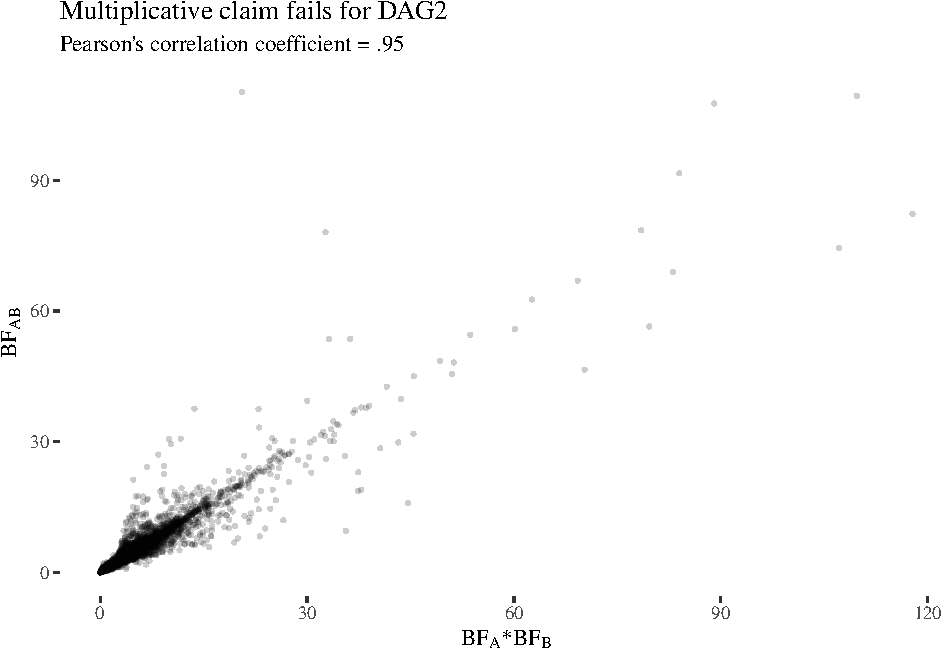
\includegraphics{BNfiles/unnamed-chunk-13-1} \end{center}

\noindent
 The scenario node unifies the different events and states.\\
Because of this unifying role, increasing the probability of one part of
the scenario (say \textsf{State/event 2}) will also increase the
probability of the other parts (\textsf{State/event 1} and
\textsf{State/event 3}). This is intended to capture the idea that the
different components of a scenario form an interconnected sequence of
events.\footnote{A discussion
of modelling crime scenarios by means of  graphical devices mixed with probabilities can be also found in the work of @shen2007ScenariodrivenDecisionSupporta},
Bex (2011), Bex (2015) and Verheij (2017). See also the survey by Di
Bello \& Verheij (2018). Dawid \& Mortera (2018) give a treatment of
scenarios in terms of Bayesian networks. Lacave \& Díez (2002)\} show
how Bayesian Network can be used to construct explanations.

Some preliminary moves towards such an explication have been made in
(Urbaniak, 2018). However, as (Neil, Fenton, Lagnado, \& Gill, 2019)
correctly points out that the paper
\texttt{fails\ to\ offer\ a\ convincing\ and\ operational\ means\ to\ structure\ and\ compare\ competing\ narratives.}

Initial philosophical analysis of the approach has been performed, (Di
Bello, 2013) pioneering a probabilistic understanding of narrations.

\todo{add more about Marcello}

\subsubsection{Impact}\label{impact}

\section{Work plan}\label{work-plan}

(general work plan, specific research goals, results of preliminary
research, risk analysis);

\section{Methodology}\label{methodology}

(underlying scientific methodology, methods, techniques and research
tools, methods of results analysis, equipment and devices to be used in
research);

\section*{References}\label{references}
\addcontentsline{toc}{section}{References}

\hypertarget{refs}{}
\hypertarget{ref-Allen1986A-Reconceptuali}{}
Allen, R. J. (1986). A reconceptualization of civil trials. \emph{Boston
University Law Review}, \emph{66}, 401--437.

\hypertarget{ref-Allen2010No-Plausible-Al}{}
Allen, R. J. (2010). No plausible alternative to a plausible story of
guilt as the rule of decision in criminal cases. In J. Cruz \& L. Laudan
(Eds.), \emph{Prueba y esandares de prueba en el derecho}. Instituto de
Investigaciones Filosoficas-UNAM.

\hypertarget{ref-allen2001naturalized}{}
Allen, R. J., \& Leiter, B. (2001). Naturalized epistemology and the law
of evidence. \emph{Virginia Law Review}, \emph{87}(8), 1491--1550.
JSTOR.

\hypertarget{ref-allen2007problematic}{}
Allen, R., \& Pardo, M. (2007). The problematic value of mathematical
models of evidence. \emph{The Journal of Legal Studies}, \emph{36}(1),
107--140. JSTOR.

\hypertarget{ref-becker1968crime}{}
Becker, G. S. (1968). Crime and punishment: An economic approach.
\emph{Journal of Political Economy}, \emph{76}, 169--217. Springer.

\hypertarget{ref-Bernoulli1713Ars-conjectandi}{}
Bernoulli, J. (1713). \emph{Ars conjectandi}.

\hypertarget{ref-bex2015IntegratedTheoryCausal}{}
Bex, F. (2015). An integrated theory of causal stories and evidential
arguments. In \emph{Proceedings of the 15th International Conference on
Artificial Intelligence and Law - ICAIL '15} (pp. 13--22). San Diego,
California: ACM Press.

\hypertarget{ref-bex2011ArgumentsStoriesCriminal}{}
Bex, F. J. (2011). \emph{Arguments, stories and criminal evidence: A
formal hybrid theory}. Law and philosophy library. Dordrecht ; New York:
Springer.

\hypertarget{ref-bovens2004bayesian}{}
Bovens, L., \& Hartmann, S. (2004). \emph{Bayesian epistemology}. Oxford
University Press.

\hypertarget{ref-brilmayer1986}{}
Brilmayer, L. (1986). Second-order evidence and bayesian logic.
\emph{Boston University Law Review}, \emph{66}, 673--691.

\hypertarget{ref-Calabresi1961}{}
Calabresi, G. (1961). Some thoughts on risk distribution and the law of
torts. \emph{Yale Law Journal}, \emph{70}, 499--553.

\hypertarget{ref-cheng2012reconceptualizing}{}
Cheng, E. (2012). Reconceptualizing the burden of proof. \emph{Yale LJ},
\emph{122}, 1254. HeinOnline.

\hypertarget{ref-clermont2015TrialTraditionalProbability}{}
Clermont, K. M. (2015). Trial by Traditional Probability, Relative
Plausibility, or Belief Function? \emph{Case Western Reserve Law
Review}, \emph{66}(2), 353--391.

\hypertarget{ref-Cohen81}{}
Cohen, J. L. (1981). Subjective probability and the paradox of the
Gatecrasher. \emph{Arizona State Law Journal}, 627--634.

\hypertarget{ref-cohen86}{}
Cohen, J. L. (1986). Twelve questions about Keynes's concept of weight.
\emph{British Journal for the Philosophy of Science}, \emph{37}(3),
263--278.

\hypertarget{ref-damaska1996free}{}
Damaška, M. R. (1995). Free proof and its detractors. \emph{The American
Journal of Comparative Law}, \emph{43}(3), 343--357.

\hypertarget{ref-dant1988gambling}{}
Dant, M. (1988). Gambling on the truth: The use of purely statistical
evidence as a basis for civil liability. \emph{Columbia Journal of Law
and Social Problems}, \emph{22}, 31--70. HeinOnline.

\hypertarget{ref-daston1988}{}
Daston, L. (1988). \emph{Classical probability in the enlightenment}.
Princeton University Press.

\hypertarget{ref-dawid1987}{}
Dawid, A. P. (1987). The difficulty about conjunction. \emph{Journal of
the Royal Statistical Society. Series D (The Statistician),}
\emph{36}(2/3), 91--92.

\hypertarget{ref-dawid2018graphical}{}
Dawid, A. P., \& Mortera, J. (2018). Graphical models for forensic
analysis. In \emph{Handbook of graphical models} (pp. 491--514). CRC
Press.

\hypertarget{ref-di2013statistics}{}
Di Bello, M. (2013). \emph{Statistics and probability in criminal
trials} (PhD thesis). University of Stanford.

\hypertarget{ref-di2018evidential}{}
Di Bello, M., \& Verheij, B. (2018). Evidential reasoning. In
\emph{Handbook of legal reasoning and argumentation} (pp. 447--493).
Springer.

\hypertarget{ref-Edwards1991Influence-diagr}{}
Edwards, W. (1991). Influence diagrams, bayesian imperialism, and the
collins case: An appeal to reason. \emph{Cardozo Law Review}, \emph{13},
1025--1074.

\hypertarget{ref-enoch2015sense}{}
Enoch, D., \& Fisher, T. (2015). Sense and sensitivity: Epistemic and
instrumental approaches to statistical evidence. \emph{Stan. L. Rev.},
\emph{67}, 557--611. HeinOnline.

\hypertarget{ref-Fenton2018Risk}{}
Fenton, N., \& Neil, M. (2018). \emph{Risk assessment and decision
analysis with bayesian networks}. Chapman; Hall.

\hypertarget{ref-fenton2013GeneralStructureLegal}{}
Fenton, N., Neil, M., \& Lagnado, D. A. (2013). A General Structure for
Legal Arguments About Evidence Using Bayesian Networks. \emph{Cognitive
Science}, \emph{37}(1), 61--102.

\hypertarget{ref-Finkelstein1970A}{}
Finkelstein, M. O., \& Fairley, W. B. (1970). A Bayesian approach to
identification evidence. \emph{Harvard Law Review}, \emph{83}(3),
489--517.

\hypertarget{ref-Franklin2001}{}
Franklin, J. (2001). \emph{The science of conjecture: Evidence and
probability before pascal}. John Hopkins University Press.

\hypertarget{ref-gaag2013elicit}{}
Gaag, L. C. van der, Renooij, S., Witteman, C. L. M., Aleman, B. M. P.,
\& Taal, B. G. (2013). How to elicit many probabilities.

\hypertarget{ref-gardiner2018}{}
Gardiner, G. (2018). Legal burdens of proof and statistical evidence. In
D. Coady \& J. Chase (Eds.), \emph{Routledge handbook of applied
epistemology}. Routledge.

\hypertarget{ref-gordon2007}{}
Gordon, T. F., Prakken, H., \& Walton, D. (2007). The Carneades model of
argument and burden of proof. \emph{Artificial Intelligence},
\emph{171}(10-15), 875--896.

\hypertarget{ref-haack2011legal}{}
Haack, S. (2014). Legal probabilism: An epistemological dissent. In
\emph{Haack2014-HAAEMS} (pp. 47--77).

\hypertarget{ref-Hacking1984}{}
Hacking, I. (1975). \emph{The emergence of probability: A philosophical
study of early ideas about probability, induction and statistical
inference}. Cambridge University Press.

\hypertarget{ref-hepler2007ObjectorientedGraphicalRepresentations}{}
Hepler, A. B., Dawid, A. P., \& Leucari, V. (2007). Object-oriented
graphical representations of complex patterns of evidence. \emph{Law,
Probability and Risk}, \emph{6}(1-4), 275--293.

\hypertarget{ref-ho2008philosophy}{}
Ho, H. L. (2008). \emph{A philosophy of evidence law: Justice in the
search for truth}. Oxford University Press.

\hypertarget{ref-kadane2011probabilistic}{}
Kadane, J. B., \& Schum, D. A. (2011). \emph{A probabilistic analysis of
the sacco and vanzetti evidence}. John Wiley \& Sons.

\hypertarget{ref-kaplow2014likelihood}{}
Kaplow, L. (2014). Likelihood ratio tests and legal decision rules.
\emph{American Law and Economics Review}, \emph{16}(1), 1--39. Oxford
University Press.

\hypertarget{ref-kaye1986admissibility}{}
Kaye, D. H. (1986). The admissibility of ``probability evidence'' in
criminal trials---part I. \emph{Jurimetrics Journal}, 343--346.

\hypertarget{ref-Kaye2010The-Double-Heli}{}
Kaye, D. H. (2010). \emph{The double helix and the law of evidence}.
Harvard University Press.

\hypertarget{ref-Koehler1996On-Conveying-th}{}
Koehler, J. J. (1996). On conveying the probative value of DNA evidence:
Frequencies, likelihood ratios, and error rates. \emph{University of
Colorado law Review}, \emph{67}, 859--886.

\hypertarget{ref-lacave2002ReviewExplanationMethodsa}{}
Lacave, C., \& Díez, F. J. (2002). A review of explanation methods for
Bayesian networks. \emph{The Knowledge Engineering Review},
\emph{17}(2), 107--127.

\hypertarget{ref-lempert1977modeling}{}
Lempert, R. O. (1977). Modeling relevance. \emph{Michigan Law Review},
\emph{75}, 1021--1057. JSTOR.

\hypertarget{ref-Lempert1986}{}
Lempert, R. O. (1986). The new evidence scholarship: Analysing the
process of proof. \emph{Boston University Law Review}, \emph{66},
439--477.

\hypertarget{ref-Lipton2004-LIPITT}{}
Lipton, P. (2004). \emph{Inference to the best explanation}.
Routledge/Taylor; Francis Group.

\hypertarget{ref-lucy2013introduction}{}
Lucy, D. (2013). \emph{Introduction to statistics for forensic
scientists}. John Wiley \& Sons.

\hypertarget{ref-NRCI1992}{}
National Research Council. (1992). \emph{DNA technology in forensic
science \textup{{[}NRC I{]}}}. Committee on DNA technology in Forensic
Science, National Research Council.

\hypertarget{ref-neil2000BuildingLargescaleBayesian}{}
Neil, M., Fenton, N., \& Nielson, L. (2000). Building large-scale
Bayesian Networks. \emph{The Knowledge Engineering Review},
\emph{15}(3), 257--284.

\hypertarget{ref-Fenton2019Modelling}{}
Neil, M., Fenton, N., Lagnado, D., \& Gill, R. D. (2019). Modelling
competing legal arguments using bayesian model comparison and averaging.
\emph{Artificial Intelligence and Law}. Retrieved from
\url{https://doi.org/10.1007/s10506-019-09250-3}

\hypertarget{ref-Nesson1979Reasonable-doub}{}
Nesson, C. R. (1979). Reasonable doubt and permissive inferences: The
value of complexity. \emph{Harvard Law Review}, \emph{92}(6),
1187--1225.

\hypertarget{ref-pardo2018}{}
Pardo, M. S. (2018). Safety vs.~Sensitivity: Possible worlds and the law
of evidence. \emph{Legal Theory}, \emph{24}(1), 50--75.

\hypertarget{ref-pardo2019}{}
Pardo, M. S. (2019). The paradoxes of legal proof: A critical guide.
\emph{Boston University Law Review}, \emph{99}(1), 233--290.

\hypertarget{ref-Pardo2008judicial}{}
Pardo, M. S., \& Allen, R. J. (2008). Judicial proof and the best
explanation. \emph{Law and Philosophy}, \emph{27}(3), 223--268.

\hypertarget{ref-Pennington1991}{}
Pennington, N., \& Hastie, R. (1991a). A cognitive theory of juror
decision making: The story model. \emph{Cardozo Law Review}, \emph{13},
519--557.

\hypertarget{ref-pennington1991cognitive}{}
Pennington, N., \& Hastie, R. (1991b). A cognitive theory of juror
decision making: The story model. \emph{Cardozo Law Review}, \emph{13},
519--557. HeinOnline.

\hypertarget{ref-pennington1992explaining}{}
Pennington, N., \& Hastie, R. (1992). Explaining the evidence: Tests of
the story model for juror decision making. \emph{Journal of personality
and social psychology}, \emph{62}(2), 189--204. American Psychological
Association.

\hypertarget{ref-Posner1973}{}
Posner, R. (1973). \emph{The economic analysis of law}. Brown \&
Company.

\hypertarget{ref-redmayne2008exploring}{}
Redmayne, M. (2008). Exploring the proof paradoxes. \emph{Legal Theory},
\emph{14}(4), 281--309. Cambridge University Press.

\hypertarget{ref-renooij2001ProbabilityElicitationBeliefa}{}
Renooij, S. (2001). Probability elicitation for belief networks: Issues
to consider. \emph{The Knowledge Engineering Review}, \emph{16}(3),
255--269.

\hypertarget{ref-Robertson1995evidence}{}
Robertson, B., \& Vignaux, G. A. (1995). DNA evidence: Wrong answers or
wrong questions? \emph{Genetica}, \emph{96}, 145--152.

\hypertarget{ref-Scutari2015Bayesian-Networ}{}
Scutari, M., \& Denis, J.-B. (2015). \emph{Bayesian networks in
\textbf{R}}. CRC Press.

\hypertarget{ref-Smith_conviction_mind_2017}{}
Smith, M. (2017). When does evidence suffice for conviction?
\emph{Mind}.

\hypertarget{ref-taroni2006bayesian}{}
Taroni, F., Biedermann, A., Bozza, S., Garbolino, P., \& Aitken, C.
(2014). \emph{Bayesian networks for probabilistic inference and decision
analysis in forensic science} (2nd ed.). John Wiley \& Sons.

\hypertarget{ref-Thomson86}{}
Thomson, J. J. (1986). Liability and individualized evidence. \emph{Law
and Contemporary Problems}, \emph{49}(3), 199--219.

\hypertarget{ref-Tillers2007}{}
Tillers, P., \& Gottfried, J. (2007). Case comment--United States v.
Copeland, 369 F. Supp. 2d 275 (E.D.N.Y. 2005): A collateral attack on
the legal maxim that proof beyond a reasonable doubt is unquantifiable?
\emph{Law, Probability and Risk}, \emph{5}(2), 135--157.

\hypertarget{ref-tribe71}{}
Tribe, L. H. (1971). Trial by mathematics: Precision and ritual in the
legal process. \emph{Harvard Law Review}, \emph{84}(6), 1329--1393.

\hypertarget{ref-Underwood1977The-thumb-on-th}{}
Underwood, B. D. (1977). The thumb on the scale of justice: Burdens of
persuasion in criminal cases. \emph{Yale Law Journal}, \emph{86(7)},
1299--1348.

\hypertarget{ref-urbaniak2018narration}{}
Urbaniak, R. (2018). Narration in judiciary fact-finding: A
probabilistic explication. \emph{Artificial Intelligence and Law},
1--32.

\hypertarget{ref-Urbaniak2019standards2}{}
Urbaniak, R. (2019). Probabilistic legal decision standards still fail.
\emph{Journal of Applied Logics}, \emph{6}(5).

\hypertarget{ref-Urbaniak2020Decision}{}
Urbaniak, R., Kowalewska, A., Janda, P., \& Dziurosz-Serafinowicz, P.
(2020). Decision-theoretic and risk-based approaches to naked
statistical evidence: Some consequences and challenges. \emph{Law,
Probability and Risk}.

\hypertarget{ref-vanEemeren2017}{}
van Eemeren, F., \& Verheij, B. (2017). Argumentation theory in formal
and computational perspective. \emph{IFCoLog Journal of Logics and Their
Applications}, \emph{4}(8), 2099--2181.

\hypertarget{ref-verheij2014catch}{}
Verheij, B. (2014). To catch a thief with and without numbers:
Arguments, scenarios and probabilities in evidential reasoning.
\emph{Law, Probability and Risk}, \emph{13}(3-4), 307--325. Citeseer.

\hypertarget{ref-verheijproof2017}{}
Verheij, B. (2017). Proof with and without probabilities. correct
evidential reasoning with presumptive arguments, coherent hypotheses and
degrees of uncertainty. \emph{Artificial Intelligence and Law}, 1--28.
Springer.

\hypertarget{ref-vlek2014building}{}
Vlek, C., Prakken, H., Renooij, S., \& Verheij, B. (2014). Building
bayesian networks for legal evidence with narratives: A case study
evaluation. \emph{Artificial Intelligence and Law}, \emph{22}, 375--421.
Springer.

\hypertarget{ref-wagenaar1993anchored}{}
Wagenaar, W., Van Koppen, P., \& Crombag, H. (1993). \emph{Anchored
narratives: The psychology of criminal evidence.} St Martin's Press.

\hypertarget{ref-Walton2002}{}
Walton, D. N. (2002). \emph{Legal argumentation and evidence}. Penn
State University Press.

\hypertarget{ref-wells1992naked}{}
Wells, G. (1992). Naked statistical evidence of liability: Is subjective
probability enough? \emph{Journal of Personality and Social Psychology},
\emph{62}(5), 739--752. American Psychological Association.

\hypertarget{ref-wigmore1901number}{}
Wigmore, J. H. (1901). Required numbers of witnesses; a brief history of
the numerical system in england. \emph{Harvard Law Review},
\emph{15}(2), 83--108.

\hypertarget{ref-wixted2017RelationshipEyewitnessConfidence}{}
Wixted, J. T., \& Wells, G. L. (2017). The Relationship Between
Eyewitness Confidence and Identification Accuracy: A New Synthesis.
\emph{Psychological Science in the Public Interest}, \emph{18}(1),
10--65.

\end{document}
